
\chapter*{Введение}
\addcontentsline{toc}{chapter}{Введение}


Феномен оценки позы человека --- это проблема, которая изучалась в течение нескольких лет, в сфере компьютерного зрения. Что же это такое? Чтобы ответить на этот вопрос, необходимо понять концепцию позы. Позу можно определить как расположение суставов человека в определенной позиции. Таким образом, мы можем определить проблему оценки позы человека как локализацию суставов человека или заранее определенных ориентиров на изображениях и видео. Существует несколько типов оценки позы, включая оценки тела, лица и рук (см. рисунок \ref{img:human,hand,face}).

\begin{figure}[ht!]
	\centering
	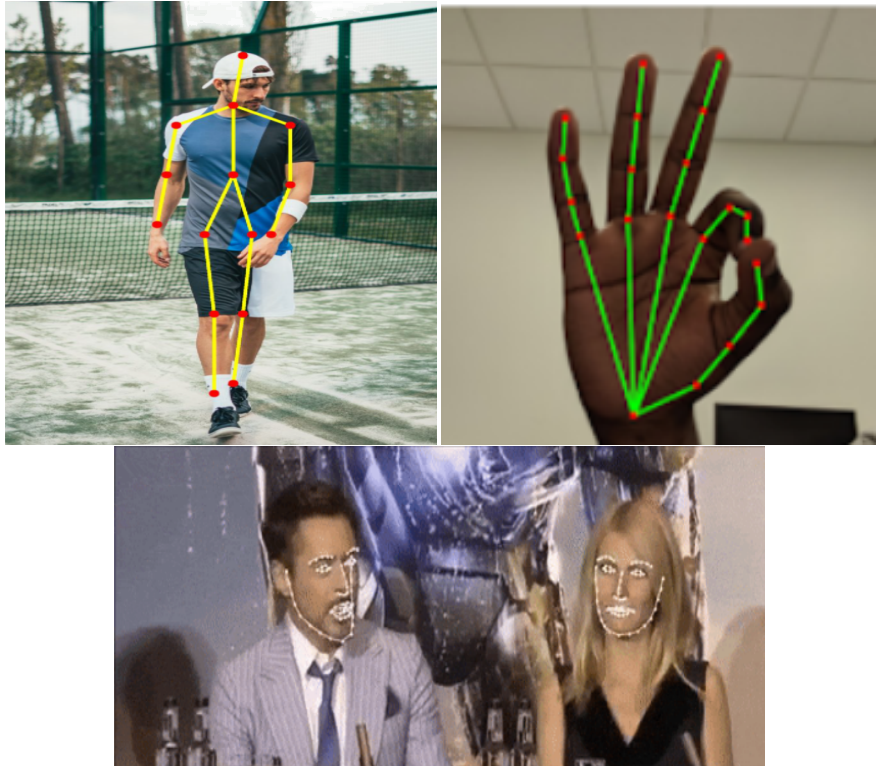
\includegraphics[width=0.96\linewidth]{assets/thefirst.png}
	\caption{Эти изображения пример разных типов определения позы человека. Верхняя левая --- это пример определения позы тела человека, верхняя правая --- это пример позы руки. Нижнее изображение --- это пример определение позы лица \cite{guide-hpe}.}
	\label{img:human,hand,face}
\end{figure}

\newpage
Целью данной работы является представить обзор и сравнение методов определения позы человека. 

Для достижения поставленной цели необходимо выполнить следующие задачи:
\begin{itemize}
	\item описать методы по определению позы человека;
	\item выбрать критерии классификации и сравнить эти методы;
	\item определить области возможного применения методов определения поз человека.
\end{itemize}